% Technologies manuscript draft prepared from:
% Target Special Issue: Advancements in Medical and Assistive Technologies Using Artificial Intelligence and Deep Learning Techniques--2nd Edition
% Format follows the provided MDPI example based on Definitions/mdpi.cls.

\documentclass[technologies,article,submit,pdftex,moreauthors]{Definitions/mdpi}

\graphicspath{{figures/}{Definitions/}}

\firstpage{1}
\makeatletter
\setcounter{page}{\@firstpage}
\makeatother
\pubvolume{1}
\issuenum{1}
\articlenumber{0}
\pubyear{2026}
\copyrightyear{2026}
\datereceived{}
\daterevised{}
\dateaccepted{}
\datepublished{}
\hreflink{https://doi.org/}

\Title{Embedded CNN--BiLSTM Myoelectric Control of a Low-Cost Robotic Hand Prosthesis: Signal Modeling, Edge Inference and Functional Validation}

\TitleCitation{Embedded CNN--BiLSTM Myoelectric Control of a Low-Cost Robotic Hand Prosthesis}

\newcommand{\orcidauthorA}{0000-0000-0000-0000}
\newcommand{\orcidauthorB}{0000-0000-0000-0000}
\newcommand{\orcidauthorC}{0000-0000-0000-0000}
\newcommand{\orcidauthorD}{0000-0000-0000-0000}
\newcommand{\orcidauthorE}{0000-0000-0000-0000}

\Author{Ronald Yessid Alvarez Suarez $^{1}$, Yennzy Camila Barrera Ardila $^{1}$, Juan Jose Lopez Mier $^{1}$, Cesar Hernando Valencia Nino $^{1,*}$ and Cristhiam Jesid Gutierrez Lozano $^{1}$}

\AuthorNames{Ronald Yessid Alvarez Suarez, Yennzy Camila Barrera Ardila, Juan Jose Lopez Mier, Cesar Hernando Valencia Nino and Cristhiam Jesid Gutierrez Lozano}

\AuthorCitation{Alvarez Suarez, R.Y.; Barrera Ardila, Y.C.; Lopez Mier, J.J.; Valencia Nino, C.H.; Gutierrez Lozano, C.J.}

\address{%
$^{1}$ \quad Faculty of Natural Sciences and Engineering, Electronic Engineering Program, Unidades Tecnologicas de Santander, Bucaramanga 680005, Colombia}

\corres{Correspondence: cesar.valencia@ustabuca.edu.co}

\abstract{Surface electromyography (sEMG) enables non-invasive prosthetic control, but practical deployment is limited by non-stationary signals, acquisition noise and embedded-computing constraints. This work presents a mathematically defined and experimentally validated pipeline for real-time control of a low-cost robotic hand prosthesis from eight-channel Myo Armband sEMG. The stream is modeled as a multichannel time series, filtered causally, segmented into overlapping windows, standardized with training-set statistics and classified by a hybrid CNN--BiLSTM model combining temporal convolutions, envelope information and bidirectional sequence modeling. Posterior probabilities are converted into prosthetic commands through temporal stabilization and a discrete gesture-to-PWM map executed on a Raspberry Pi with TensorFlow Lite and a PCA9685 driver. Five classes were considered: rest, open hand, closed fist, pinch and object grasp. From 167,712 labeled samples, the model achieved 99.6\% test accuracy and 99.58\% macro F1-score over 496 test windows. During embedded operation, 199 predictions were generated in 44.5 s, with mean confidence of 0.9015, median confidence of 0.9589 and temporal stability of 88.9\%. Functional validation confirmed coherent gesture-to-motion mapping. The results support edge-deployed deep learning for affordable myoelectric assistive technologies while highlighting the need for multi-user, cross-session and amputee-user validation.}

\keyword{surface electromyography; robotic prosthesis; deep learning; CNN-BiLSTM; TensorFlow Lite; embedded systems; assistive technology; gesture recognition; myoelectric control}

\begin{document}

\section{Introduction}

Upper-limb prosthetic control is a central problem in assistive technologies because it determines whether an artificial limb becomes an active functional interface. Surface electromyography (sEMG) is relevant because it records residual muscle activity non-invasively and can infer movement intention \cite{Farina2014,Englehart2003,Hudgins1993,Ha2011,Kuiken2009,Cipriani2011}. The difficulty is that sEMG is not a stationary command signal: amplitude and spectral content vary with electrode placement, contraction intensity, fatigue, skin impedance, limb posture and motion artifacts \cite{Oskoei2007,Scheme2011,Chowdhury2013,Merletti1997}. A prosthetic controller must therefore estimate gesture intention from short noisy temporal observations and convert that estimate into stable actuator commands. Deep-learning models are attractive because convolutional and recurrent layers can learn discriminative representations directly from multichannel EMG windows \cite{LeCun2015,Hochreiter1997,Tsinganos2018,Celik2026,Shanmuganathan2023}.

However, high offline accuracy is not sufficient for assistive-device relevance. A classifier that performs well on stored windows may fail in a portable system because acquisition jitter, filter states, inference time, power-supply disturbances and actuator dynamics enter the sensing--inference--actuation chain. Recent work in \textit{Technologies} has emphasized AI, embedded implementation, robotics, rehabilitation and sensor-driven healthcare systems \cite{Dunai2025Tech,Covaciu2025Tech,Lotfi2018Tech,Stasolla2023Tech,Bush2024Tech,Giansanti2025Tech,Manakitsa2024Tech,Percuku2025Tech,Jalloul2025Tech,Kouretas2020Tech,Kraft2020Tech,Sanida2022Tech}, which aligns with the present focus on an edge-deployable myoelectric prosthesis rather than only an offline classifier.

The research question addressed in this paper is therefore: \textit{Can a low-cost embedded platform execute a reproducible sEMG sensing--inference--actuation pipeline that preserves high intra-subject gesture-classification performance while maintaining stable real-time prosthetic commands?} The working hypothesis is that a hybrid CNN--BiLSTM model, when coupled with causal preprocessing, window-level normalization, temporal decision stabilization and progressive PWM actuation, can provide both high offline classification performance and stable embedded operation under controlled intra-subject conditions.

This work addresses that question through a Myo Armband, Raspberry Pi, hybrid CNN--BiLSTM classifier and PWM-driven five-finger robotic hand. The specific contributions are:

\begin{itemize}
    \item a formal signal-processing and control formulation for transforming streaming eight-channel sEMG into stabilized prosthetic commands;
    \item a hybrid CNN--BiLSTM classifier that combines local temporal convolutions, EMG-envelope features and bidirectional temporal modeling;
    \item an embedded TensorFlow Lite implementation with asynchronous acquisition, online filtering, sliding-window inference and PCA9685-based PWM actuation;
    \item quantitative validation of offline classification performance, online confidence, temporal stability and functional gesture-to-motion correspondence.
\end{itemize}

The paper is organized as follows: Section~2 reviews the literature; Section~3 presents the proposed embedded myoelectric-control framework; Section~4 describes the experimental materials, model and metrics; Section~5 reports validation results; Section~6 discusses implications and limitations; and Section~7 concludes the study.

\section{Literature Review}

\subsection{sEMG-Based Prosthetic Control}

Myoelectric control has evolved from early multifunction strategies to modern pattern-recognition systems \cite{Hudgins1993,Englehart2003,Oskoei2007,Scheme2011}. Residual muscle activity contains movement-intention information, but reliability depends on acquisition conditions, electrode placement and temporal variability \cite{Farina2014,Chowdhury2013,Merletti1997}. High-performance control must therefore address classification, real-time usability, command stability and interaction with the physical prosthesis \cite{Kuiken2009,Cipriani2011,Ha2011}.

\subsection{Wearable EMG Acquisition and the Myo Armband}

Wearable armbands have made multichannel EMG acquisition accessible for research prototypes. The Myo Armband has been used in gesture recognition, physiotherapy and machine-learning studies because it provides compact eight-channel wireless acquisition \cite{He2017Myo,Kaya2018Myo,Sathiyanarayanan2016Myo,Boyali2015Myo,Benalcazar2017Myo}. Its limitations--sampling rate, electrode geometry, packet timing and placement sensitivity--make reproducible filtering, segmentation, normalization and labeling essential.

\subsection{Deep Learning for EMG Gesture Recognition}

Deep-learning methods learn temporal and spatial representations from multichannel windows without relying exclusively on hand-crafted features \cite{LeCun2015,Tsinganos2018,Nahid2020Myo,Chung2019Myo,Celik2026}. Convolutions capture local activation patterns, whereas LSTMs model within-window sequence dependencies \cite{Hochreiter1997}. Because controlled intra-subject data can inflate offline performance, prosthetic studies should complement accuracy with embedded-operation analysis.

\subsection{Embedded AI and Assistive Technologies}

Recent articles in \textit{Technologies} report AI, embedded, robotic and assistive systems for healthcare, rehabilitation, sensing and edge computing \cite{Dunai2025Tech,Covaciu2025Tech,Lotfi2018Tech,Stasolla2023Tech,Bush2024Tech,Giansanti2025Tech,Manakitsa2024Tech,Percuku2025Tech,Jalloul2025Tech,Kouretas2020Tech,Kraft2020Tech,Sanida2022Tech}. The remaining gap addressed here is the integration of wearable sEMG acquisition, mathematically specified preprocessing, embedded CNN--BiLSTM inference and physical PWM prosthetic actuation in one low-cost prototype.

\section{Proposed Embedded Myoelectric-Control Framework}

\subsection{Framework Architecture}

The proposed human-machine interface converts forearm muscle activity into robotic-hand actions through seven linked stages: sEMG acquisition, causal preprocessing, window construction, CNN-envelope feature extraction, BiLSTM inference, temporal decision stabilization and PWM prosthetic actuation. A Raspberry Pi receives the wireless stream, executes TensorFlow Lite inference and communicates with the actuation stage. Acquisition, filtering, inference and actuation are decoupled through buffers and queues to reduce blocking during real-time operation. The complete computational framework is shown in Figure~\ref{fig:proposed-framework}, and the integrated hardware is shown in Figure~\ref{fig:system-integration}.

\begin{figure}[H]
\centering
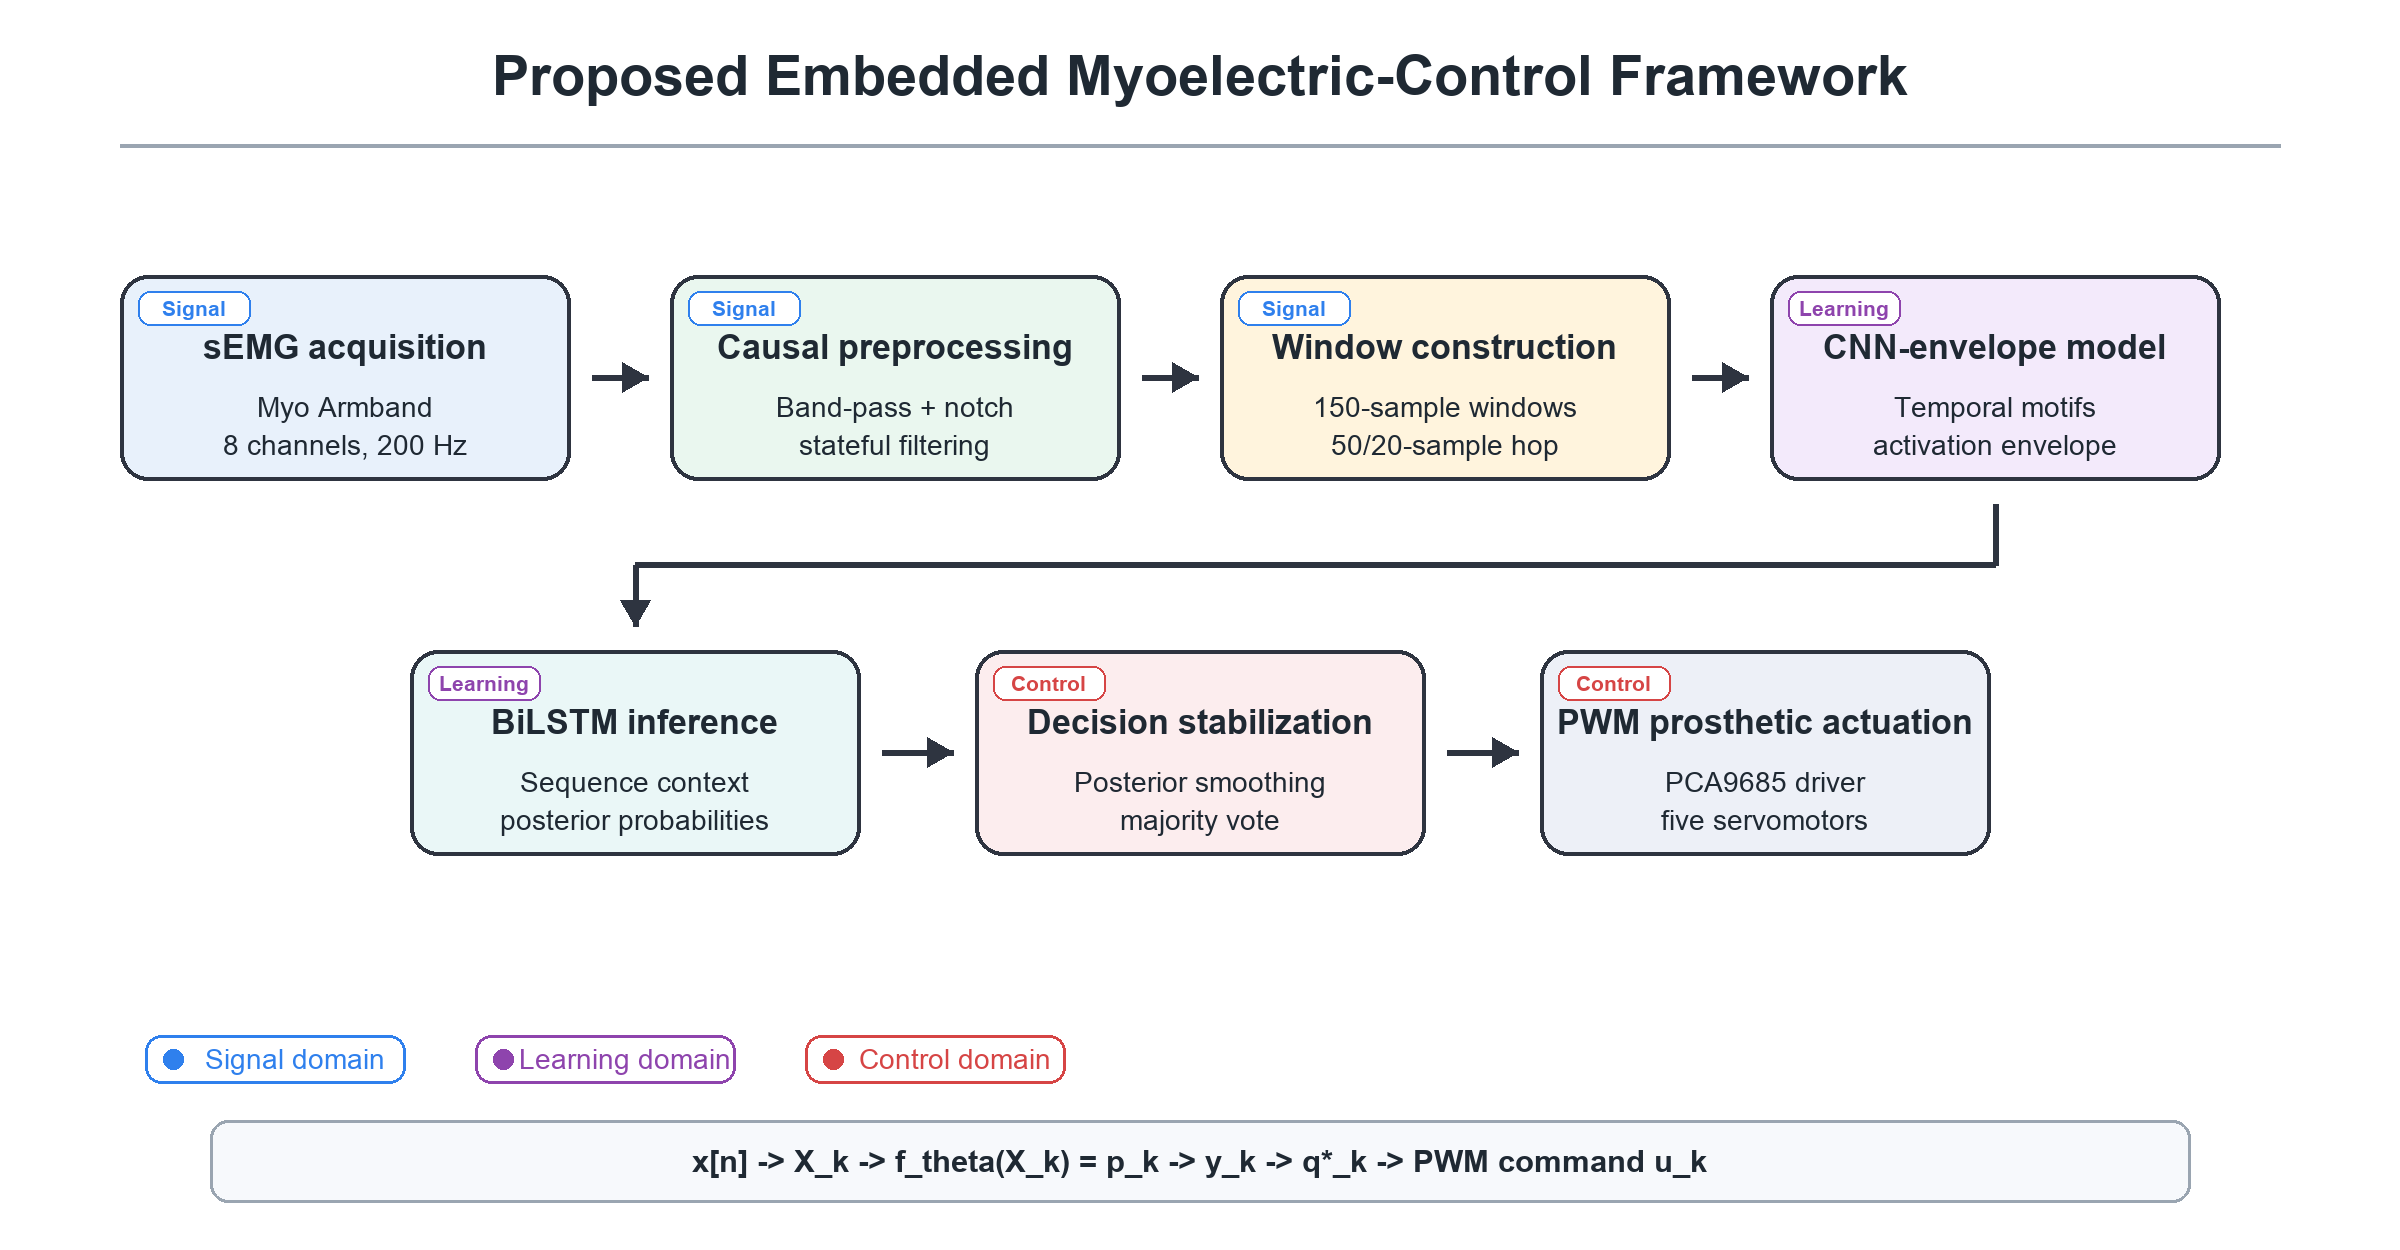
\includegraphics[width=0.98\linewidth]{fig08_proposed_framework.png}
\caption{Proposed embedded myoelectric-control framework. The pipeline connects multichannel sEMG acquisition, causal filtering, sliding-window construction, hybrid CNN--BiLSTM inference, temporal decision stabilization and PWM prosthetic actuation in a single edge-deployed assistive system.\label{fig:proposed-framework}}
\end{figure}

\begin{figure}[H]
\centering
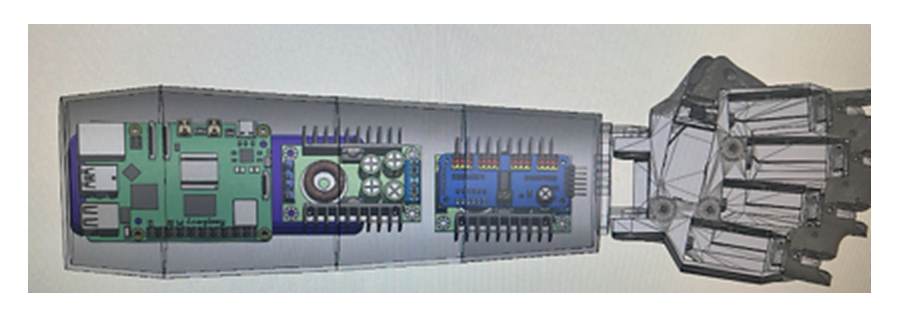
\includegraphics[width=0.88\linewidth]{fig00_system_integration.png}
\caption{Integrated robotic-hand system showing the embedded processing unit, actuation electronics and mechanical hand assembly. The prototype closes the loop from EMG interpretation to physical hand movement.\label{fig:system-integration}}
\end{figure}

\subsection{Mathematical Formulation of the Myoelectric-Control Pipeline}

Let the acquired sEMG stream be represented as a discrete multichannel sequence
\begin{equation}
    \label{eq:semg-stream}
    \mathbf{x}[n] = \left[x_1[n],x_2[n],\ldots,x_C[n]\right]^{\top} \in \mathbb{R}^{C},
    \quad C=8,
\end{equation}
where $n$ is the sample index and $C$ is the number of Myo Armband channels. At the sensor level, the measured signal can be interpreted as a spatially mixed observation of latent neuromuscular sources contaminated by physiological noise, motion artifacts and acquisition interference:
\begin{equation}
    \label{eq:semg-generative}
    \mathbf{x}[n]
    =
    \mathbf{A}\mathbf{s}[n]
    +
    \boldsymbol{\eta}[n]
    +
    \boldsymbol{\nu}[n],
\end{equation}
where $\mathbf{s}[n]$ denotes latent muscle sources, $\mathbf{A}$ is an unknown spatial mixing matrix, $\boldsymbol{\eta}[n]$ represents biological and motion variability, and $\boldsymbol{\nu}[n]$ accounts for acquisition interference. Equation~\eqref{eq:semg-generative} motivates multichannel learning because gesture information is distributed across time and channels.

The acquisition process defines a supervised sequence-labeling problem in which each temporal segment must be assigned to one of $M=5$ gesture classes,
\begin{equation}
    \label{eq:gesture-set}
    \mathcal{Y}=\{\text{rest}, \text{open hand}, \text{closed fist}, \text{pinch}, \text{object grasp}\}.
\end{equation}
The class set in Equation~\eqref{eq:gesture-set} was selected to cover rest, hand opening, power closure and two functional grasping patterns.

After online filtering, the continuous stream is segmented into overlapping windows
\begin{equation}
    \label{eq:windowing}
    \mathbf{X}_k =
    \left[
    \mathbf{x}[kH],\mathbf{x}[kH+1],\ldots,\mathbf{x}[kH+W-1]
    \right]^{\top}
    \in \mathbb{R}^{W \times C},
\end{equation}
where $W=150$ samples and $H$ is the hop size. Training used $H=50$; embedded inference used $H=20$, equivalent to approximately 0.1 s at 200 Hz. Each window is standardized using training-set statistics:
\begin{equation}
    \label{eq:zscore}
    \tilde{x}_{c}[n]=\frac{x_c[n]-\mu_c}{\sigma_c+\epsilon},
    \quad c=1,\ldots,C,
\end{equation}
where $\mu_c$ and $\sigma_c$ are the training-set mean and standard deviation of channel $c$, and $\epsilon$ is a small constant used to avoid numerical instability.

The classifier is a parametric function $f_{\boldsymbol{\theta}}:\mathbb{R}^{W\times C}\rightarrow[0,1]^M$ that produces the posterior probability vector
\begin{equation}
    \label{eq:posterior}
    \mathbf{p}_k=f_{\boldsymbol{\theta}}(\tilde{\mathbf{X}}_k),
    \quad
    \sum_{m=1}^{M}p_{k,m}=1.
\end{equation}
The discriminative decision problem is
\begin{equation}
    \label{eq:bayes-decision}
    \hat{y}_k
    =
    \arg\max_{y\in\mathcal{Y}}
    P\left(y\mid \tilde{\mathbf{X}}_k;\boldsymbol{\theta}\right),
\end{equation}
implemented through Equation~\eqref{eq:posterior}; equivalently,
\begin{equation}
    \label{eq:argmax}
    \hat{y}_k = \arg\max_{m \in \{1,\ldots,M\}} p_{k,m}.
\end{equation}

Two temporal decision operators reduce isolated real-time errors. The first smooths the posterior vectors over the last $K=7$ predictions:
\begin{equation}
    \label{eq:posterior-smoothing}
    \bar{\mathbf{p}}_k
    =
    \frac{1}{K}
    \sum_{j=0}^{K-1}
    \mathbf{p}_{k-j},
    \quad
    \tilde{y}_k = \arg\max_m \bar{p}_{k,m}.
\end{equation}
The second applies majority voting:
\begin{equation}
    \label{eq:majority-vote}
    \bar{y}_k =
    \operatorname{mode}\left(
    \hat{y}_{k-K+1},\ldots,\hat{y}_{k}
    \right).
\end{equation}
Equations~\eqref{eq:bayes-decision}, \eqref{eq:argmax}, \eqref{eq:posterior-smoothing} and~\eqref{eq:majority-vote} define the decision layer.
The stabilized class $\bar{y}_k$ is then mapped to a desired actuator-position vector
\begin{equation}
    \label{eq:gesture-map}
    \mathbf{q}^{\star}_k = \mathbf{Q}_{\bar{y}_k}
    =
    \left[q^{\star}_{1,k},q^{\star}_{2,k},\ldots,q^{\star}_{5,k}\right]^{\top},
\end{equation}
where $\mathbf{Q}_{\bar{y}_k}$ in Equation~\eqref{eq:gesture-map} is the predefined five-servo configuration associated with the detected gesture. Servo commands are generated through PWM pulses bounded by the calibrated actuator range,
\begin{equation}
    \label{eq:pwm-map}
    u_{i,k}=
    u^{\min}_{i}
    +
    \frac{q^{\star}_{i,k}-q^{\min}_{i}}{q^{\max}_{i}-q^{\min}_{i}}
    \left(u^{\max}_{i}-u^{\min}_{i}\right),
    \quad i=1,\ldots,5,
\end{equation}
with typical pulse widths between 1 and 2 ms over a 20 ms period; Equation~\eqref{eq:pwm-map} therefore maps desired finger position to electrical command. The controller updates the servo state by incremental interpolation,
\begin{equation}
    \label{eq:pwm-interpolation}
    \mathbf{q}_{k+1}=\mathbf{q}_{k}+\alpha\left(\mathbf{q}^{\star}_{k}-\mathbf{q}_{k}\right),
    \quad 0<\alpha\leq1,
\end{equation}
which reduces abrupt movements and current peaks. A safety-oriented motion bound is
\begin{equation}
    \label{eq:servo-rate-limit}
    \left\|\mathbf{q}_{k+1}-\mathbf{q}_{k}\right\|_{\infty}
    \leq
    \Delta q_{\max},
\end{equation}
where $\Delta q_{\max}$ is the maximum permitted per-update servo-position change. Equations~\eqref{eq:pwm-interpolation} and~\eqref{eq:servo-rate-limit} define bounded discrete-time prosthetic motion.

Equations~\eqref{eq:semg-stream}--\eqref{eq:servo-rate-limit} define the path from sEMG acquisition to actuator command generation and fix the window length, normalization constants, decision rule and servo-command mapping.

\section{Experimental Materials and Methods}

\subsection{Acquisition Hardware and Experimental Protocol}

sEMG signals were acquired with an eight-channel Myo Armband placed circumferentially around the forearm and connected to the Raspberry Pi through Bluetooth Low Energy and a BLED112 dongle. The approximate sampling frequency was 200 Hz per channel. The device was selected because it is compact, wearable and widely used in gesture-recognition and rehabilitation studies \cite{He2017Myo,Kaya2018Myo,Sathiyanarayanan2016Myo,Boyali2015Myo,Benalcazar2017Myo}. Each BLE packet was decoded as
\begin{equation}
    \label{eq:csv-row}
    \mathbf{r}_n =
    \left[t_n, x_1[n],x_2[n],\ldots,x_8[n], y_n\right],
\end{equation}
where $t_n$ is the timestamp and $y_n$ is the gesture label. Equation~\eqref{eq:csv-row} permits time-series reconstruction, packet inspection and supervised segmentation into Equation~\eqref{eq:windowing}.

One participant performed rest, open hand, closed fist, pinch and object grasp under informed consent and Declaration of Helsinki principles. Before each session, BLED112 detection, BLE stability and activity in all channels were verified; the armband orientation was kept consistent; and the participant remained seated with supported forearm and neutral wrist. An interactive Raspberry Pi interface synchronized labels with acquisition intervals. Segments with inactive channels, excessive noise or inconsistent labels were discarded. Figure~\ref{fig:emg-acquisition} shows the monitoring interface.

\begin{figure}[H]
\centering
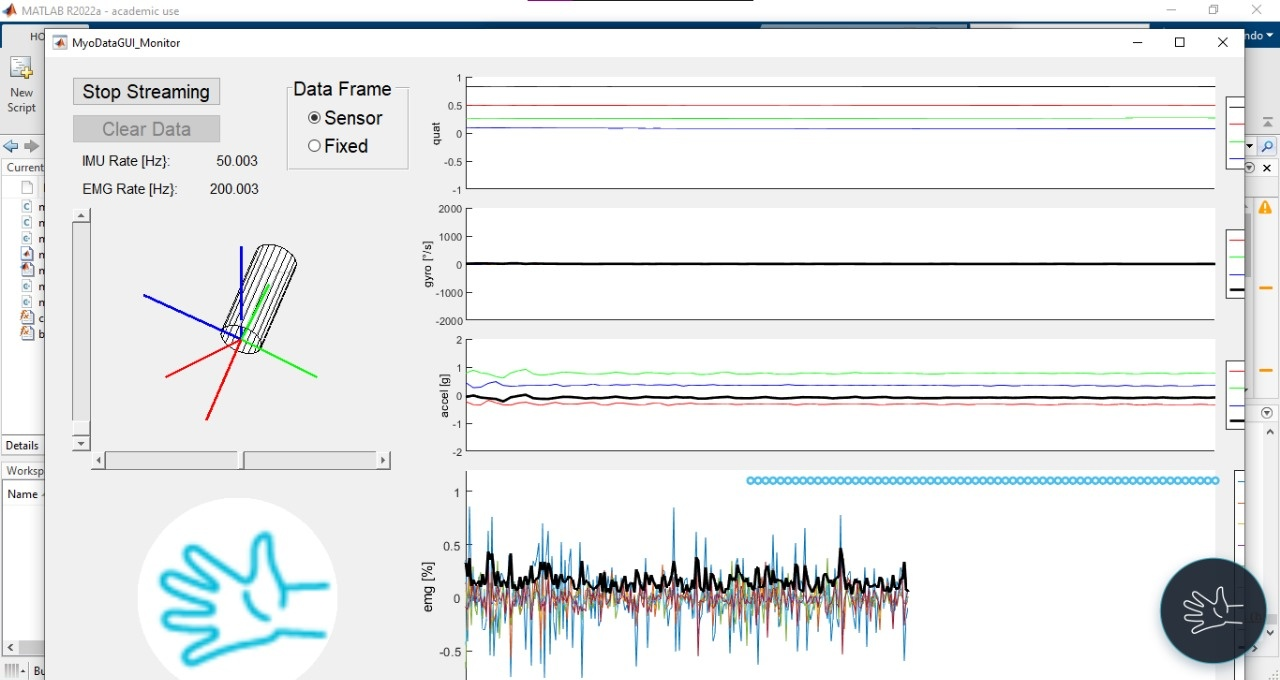
\includegraphics[width=0.86\linewidth]{fig01_emg_acquisition.jpeg}
\caption{Experimental acquisition and visualization of multichannel EMG signals from the Myo Armband during hand-gesture execution. The setup supports real-time monitoring of differential activation patterns before dataset construction.\label{fig:emg-acquisition}}
\end{figure}

\subsection{Signal Preprocessing and Segmentation}

The preprocessing chain was designed to preserve physiologically relevant information while reducing acquisition noise and preparing the data for deep-learning inference. Each raw channel was processed by a causal band-pass filter and two notch filters. In compact form, the filtered stream can be expressed as
\begin{equation}
    \label{eq:filter-chain}
    \mathbf{x}_{f}[n]
    =
    \mathcal{H}_{60}
    \left\{
    \mathcal{H}_{50}
    \left[
    \mathcal{H}_{\mathrm{bp}}\left(\mathbf{x}[n]\right)
    \right]
    \right\},
\end{equation}
where $\mathcal{H}_{\mathrm{bp}}$ denotes the 20--450 Hz band-pass operation, and $\mathcal{H}_{50}$ and $\mathcal{H}_{60}$ denote notch attenuation at 50 and 60 Hz, respectively. The band-pass range was selected to retain the dominant physiological content of sEMG while attenuating low-frequency motion artifacts and high-frequency noise.

Filtering used recursive structures that preserve internal state for streaming operation. The filtered signal was segmented into 150-sample windows, equivalent to 0.75 s at 200 Hz, with 50-sample training hops and 20-sample inference hops. Each model input was therefore a $150 \times 8$ matrix.

Z-score parameters were computed only from the training subset and applied to validation, test and real-time data to avoid leakage. This preprocessing is critical because EMG classification is strongly affected by signal quality \cite{Phinyomark2012,Atzori2014SciData,NinaPro2015,Muceli2013,Prakash2021}.

The trained model was stored with channel-wise means and standard deviations, class mapping, filter configuration, window length, hops and majority-vote length, preventing train-deployment mismatch in Equations~\eqref{eq:filter-chain} and~\eqref{eq:zscore}.

In addition to the filtered waveform, amplitude descriptors were computed to represent the local recruitment intensity of the forearm muscles. The moving-average rectified envelope for channel $c$ was defined as
\begin{equation}
    \label{eq:emg-envelope}
    e_c[n]
    =
    \frac{1}{L}
    \sum_{r=0}^{L-1}
    \left|x_{f,c}[n-r]\right|,
\end{equation}
where $L$ is the envelope-smoothing length. A window-level RMS descriptor was also used to quantify the effective activation energy of each channel:
\begin{equation}
    \label{eq:rms-feature}
    \mathrm{RMS}_{c,k}
    =
    \sqrt{
    \frac{1}{W}
    \sum_{r=0}^{W-1}
    x_{f,c}^{2}[kH+r]
    }.
\end{equation}
Equations~\eqref{eq:emg-envelope} and~\eqref{eq:rms-feature} formalize the physiological information represented by the envelope branch and provide interpretable quantities for reproducibility.

\subsection{Dataset}

The complete dataset contained 167,712 instantaneous sEMG samples distributed across the five gesture classes. Table~\ref{tab:class_distribution} summarizes the sample distribution.

\begin{table}[H]
\centering
\caption{Distribution of samples by gesture class in the complete dataset.\label{tab:class_distribution}}
\begin{tabular}{lc}
\toprule
\textbf{Gesture class} & \textbf{Number of samples} \\
\midrule
Object grasp & 35,940 \\
Open hand & 23,956 \\
Pinch & 47,914 \\
Closed fist & 23,958 \\
Rest & 35,944 \\
\midrule
Total & 167,712 \\
\bottomrule
\end{tabular}
\end{table}

The dataset was divided into training, validation and test subsets using a stratified 70/15/15 split, preserving class proportions across partitions (Table~\ref{tab:split_distribution}).
The split was performed within the controlled intra-subject acquisition domain; therefore, test performance quantifies same-subject feasibility under the described protocol rather than cross-user or cross-session generalization.

\begin{table}[H]
\centering
\caption{Stratified partition of the dataset.\label{tab:split_distribution}}
\begin{tabular}{lcc}
\toprule
\textbf{Subset} & \textbf{Percentage} & \textbf{Number of samples} \\
\midrule
Training & 70\% & 117,398 \\
Validation & 15\% & 25,157 \\
Test & 15\% & 25,157 \\
\midrule
Total & 100\% & 167,712 \\
\bottomrule
\end{tabular}
\end{table}

Table~\ref{tab:reproducibility_parameters} summarizes the main experimental and computational parameters required to reproduce the proposed pipeline.

\begin{table}[H]
\centering
\caption{Key reproducibility parameters of the proposed myoelectric-control pipeline.\label{tab:reproducibility_parameters}}
\begin{tabularx}{0.94\linewidth}{lX}
\toprule
\textbf{Component} & \textbf{Configuration} \\
\midrule
sEMG sensor & Myo Armband, 8 channels \\
Sampling frequency & Approximately 200 Hz per channel \\
Gesture classes & Rest, open hand, closed fist, pinch, object grasp \\
Band-pass filtering & 20--450 Hz \\
Notch filtering & 50 Hz and 60 Hz \\
Training window & 150 samples, 50-sample hop \\
Embedded inference window & 150 samples, 20-sample hop \\
Input tensor & $150 \times 8$ \\
Normalization & Z-score using training-set statistics \\
Classifier & CNN--BiLSTM with envelope branch \\
Training objective & Weighted categorical cross-entropy with label smoothing \\
Optimizer & Adam, initial learning rate $10^{-3}$ \\
Regularization & Dropout 0.3, early stopping, class weighting \\
Embedded model & TensorFlow Lite, FP16 optimization \\
Decision stabilization & Majority vote over $K=7$ predictions \\
Actuation & PCA9685 PWM driver, five MG90S servomotors \\
Control update & Progressive PWM interpolation \\
\bottomrule
\end{tabularx}
\end{table}

\subsection{CNN--BiLSTM Architecture}

The classifier combines convolutional, envelope-based and recurrent processing from a $150 \times 8$ EMG window. For a convolutional layer, the feature map is
\begin{equation}
    \label{eq:conv1d}
    \mathbf{z}^{(\ell)}_{t,j}
    =
    \phi
    \left(
    \sum_{r=0}^{R_{\ell}-1}
    \sum_{d=1}^{D_{\ell-1}}
    w^{(\ell)}_{r,d,j}
    \mathbf{z}^{(\ell-1)}_{t-r,d}
    + b^{(\ell)}_{j}
    \right),
\end{equation}
where $R_{\ell}$ is the kernel length, $D_{\ell-1}$ is the input depth, $j$ indexes output filters and $\phi(\cdot)$ is ReLU after batch normalization.

In parallel, an envelope branch computes $|\tilde{\mathbf{X}}_k|$, applies moving-average smoothing and extracts activation-intensity features. The convolutional and envelope representations are concatenated and passed to a BiLSTM layer with forward and backward hidden states,
\begin{equation}
    \label{eq:bilstm-state}
    \mathbf{h}_{t}
    =
    \left[
    \overrightarrow{\mathbf{h}}_{t};
    \overleftarrow{\mathbf{h}}_{t}
    \right],
\end{equation}
so that the representation summarizes temporal dependencies in both directions. A dropout layer and softmax dense layer perform classification:
\begin{equation}
    \label{eq:softmax}
    p_{k,m}
    =
    \frac{\exp(a_{k,m})}
    {\sum_{j=1}^{M}\exp(a_{k,j})}.
\end{equation}

\begin{table}[H]
\centering
\caption{CNN--BiLSTM architecture used for sEMG gesture classification.\label{tab:architecture}}
\begin{tabular}{llll}
\toprule
\textbf{Layer} & \textbf{Type} & \textbf{Parameters} & \textbf{Output} \\
\midrule
1 & Input & EMG window & $(150, 8)$ \\
2 & Conv1D & 32 filters, kernel 7, no bias & $(150, 32)$ \\
3 & Batch normalization & -- & $(150, 32)$ \\
4 & ReLU & -- & $(150, 32)$ \\
5 & Conv1D & 64 filters, kernel 5, no bias & $(150, 64)$ \\
6 & Batch normalization & -- & $(150, 64)$ \\
7 & ReLU & -- & $(150, 64)$ \\
8 & Envelope branch & $|x|$ & $(150, 8)$ \\
9 & AvgPooling1D & pool 5, stride 1 & $(150, 8)$ \\
10 & Conv1D & 16 filters, kernel 3 & $(150, 16)$ \\
11 & Concatenation & 64 + 16 channels & $(150, 80)$ \\
12 & BiLSTM & 64 units, unroll=True & $(128)$ \\
13 & Dropout & 0.3 & $(128)$ \\
14 & Dense & softmax, 5 classes & $(5)$ \\
\bottomrule
\end{tabular}
\end{table}

Table~\ref{tab:architecture} and Figure~\ref{fig:model-architecture} report the architecture. The BiLSTM was explicitly unrolled to facilitate TensorFlow Lite conversion for Raspberry Pi deployment.

\begin{figure}[H]
\centering
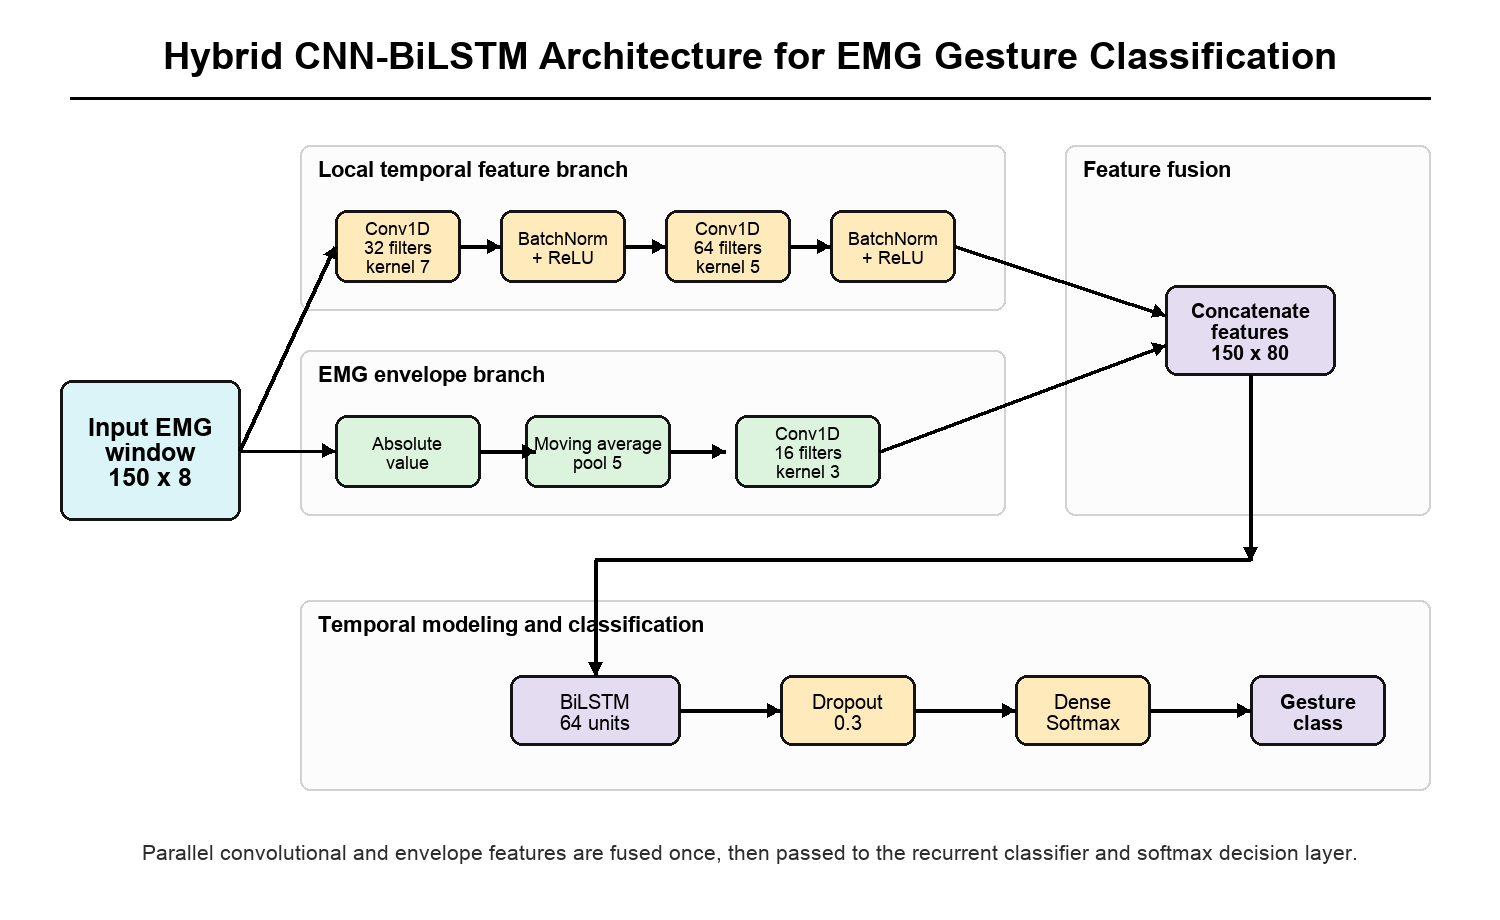
\includegraphics[width=0.88\linewidth]{fig02_cnn_bilstm_architecture.png}
\caption{Hybrid CNN--BiLSTM model used for EMG gesture classification. The architecture combines local convolutional features, an EMG-envelope branch and bidirectional temporal modeling before softmax classification.\label{fig:model-architecture}}
\end{figure}

\subsection{Training Procedure}

The model was trained with Adam, initial learning rate $10^{-3}$, batch size 128 and maximum 60 epochs. Let $\mathbf{y}_i$ be the one-hot label and $\mathbf{p}_i$ the predicted probability vector. With label smoothing coefficient $\lambda$,
\begin{equation}
    \label{eq:label-smoothing}
    y'_{i,m}=(1-\lambda)y_{i,m}+\frac{\lambda}{M},
    \quad \lambda=0.05.
\end{equation}
The weighted training objective is
\begin{equation}
    \label{eq:training-loss}
    \mathcal{L}(\boldsymbol{\theta})
    =
    -\frac{1}{N}
    \sum_{i=1}^{N}
    \omega_{y_i}
    \sum_{m=1}^{M}
    y'_{i,m}
    \log\left(p_{i,m}\right),
\end{equation}
where $\omega_{y_i}$ is the inverse-frequency class weight. Early stopping with patience 12 and adaptive learning-rate reduction were used.

The trained model was exported as Keras/HDF5 and TensorFlow Lite with FP16 optimization \cite{Zaman2020TFLite}.

The training objective is one component of a broader myoelectric-control criterion:
\begin{equation}
    \label{eq:system-objective}
    \mathcal{J}
    =
    \mathcal{L}(\boldsymbol{\theta})
    +
    \beta
    \sum_{k}
    \left\|\mathbf{p}_{k}-\mathbf{p}_{k-1}\right\|_{2}^{2}
    +
    \rho
    \sum_{k}
    \left\|\mathbf{q}_{k+1}-\mathbf{q}_{k}\right\|_{2}^{2}.
\end{equation}
In Equation~\eqref{eq:system-objective}, the first term is the supervised loss, the second penalizes posterior instability and the third penalizes abrupt servo motion. The first was optimized during training; the last two were enforced through smoothing, voting and PWM interpolation.

Equations~\eqref{eq:conv1d}, \eqref{eq:bilstm-state}, \eqref{eq:softmax}, \eqref{eq:label-smoothing}, \eqref{eq:training-loss} and~\eqref{eq:system-objective} specify feature extraction, temporal representation, posterior estimation and deployment-oriented smoothness.

\subsection{Computational Complexity and Embedded Latency}

The architecture was constrained by embedded execution. For a Conv1D layer, leading-order complexity is
\begin{equation}
    \label{eq:conv-complexity}
    \mathcal{O}_{\mathrm{conv}}
    =
    T R D_{\mathrm{in}}D_{\mathrm{out}}.
\end{equation}
For an LSTM layer,
\begin{equation}
    \label{eq:lstm-complexity}
    \mathcal{O}_{\mathrm{LSTM}}
    =
    4T h(h+d+1),
\end{equation}
where the factor four accounts for the input, forget, output and candidate gates. Equations~\eqref{eq:conv-complexity} and~\eqref{eq:lstm-complexity} justify a compact CNN--BiLSTM because inference shares processor time with acquisition, filtering, decision logic and actuation.

End-to-end response time was modeled as
\begin{equation}
    \label{eq:latency-budget}
    T_{\mathrm{total}}
    =
    T_{\mathrm{win}}
    +
    T_{\mathrm{pre}}
    +
    T_{\mathrm{inf}}
    +
    T_{\mathrm{dec}}
    +
    T_{\mathrm{act}},
\end{equation}
where the terms denote window acquisition, preprocessing, inference, decision and actuation times. For interactive use,
\begin{equation}
    \label{eq:latency-constraint}
    T_{\mathrm{total}} < T_{\max},
\end{equation}
where $T_{\max}$ is the maximum acceptable response time. Equations~\eqref{eq:latency-budget} and~\eqref{eq:latency-constraint} connect model selection and scheduling to responsive prosthetic behavior.

\subsection{Embedded Real-Time Inference}

In real time, the Raspberry Pi filters the sEMG stream, updates a circular buffer and forms windows while TensorFlow Lite inference runs in an independent thread. Each prediction includes a class and confidence
\begin{equation}
    \label{eq:confidence}
    \gamma_k = \max_m p_{k,m}.
\end{equation}
Confidence is used as an implementation-level certainty indicator, not as a clinical reliability measure.

Prediction uncertainty was also quantified using the Shannon entropy of the posterior distribution:
\begin{equation}
    \label{eq:posterior-entropy}
    H(\mathbf{p}_k)
    =
    -
    \sum_{m=1}^{M}
    p_{k,m}\log(p_{k,m}).
\end{equation}
Low entropy indicates concentrated probability mass; high entropy indicates ambiguity during transitions, partial contractions or unstable armband contact.

Temporal smoothing uses Equations~\eqref{eq:posterior-smoothing} and~\eqref{eq:majority-vote}; the controller acts on the smoothed class to suppress short-lived fluctuations.

\subsection{Robotic Prosthesis and PWM Control}

The robotic hand was based on the open-source InMoov Hand i2 design, with a custom CAD forearm housing. Structural elements were fabricated in PLA and finger components in resin. Five MG90S servomotors actuated tendon-like nylon lines, and a PCA9685 controller generated 1--2 ms servo pulses over a 20 ms period. Component groups are summarized in Figure~\ref{fig:prosthesis-components}.

\begin{figure}[H]
\centering
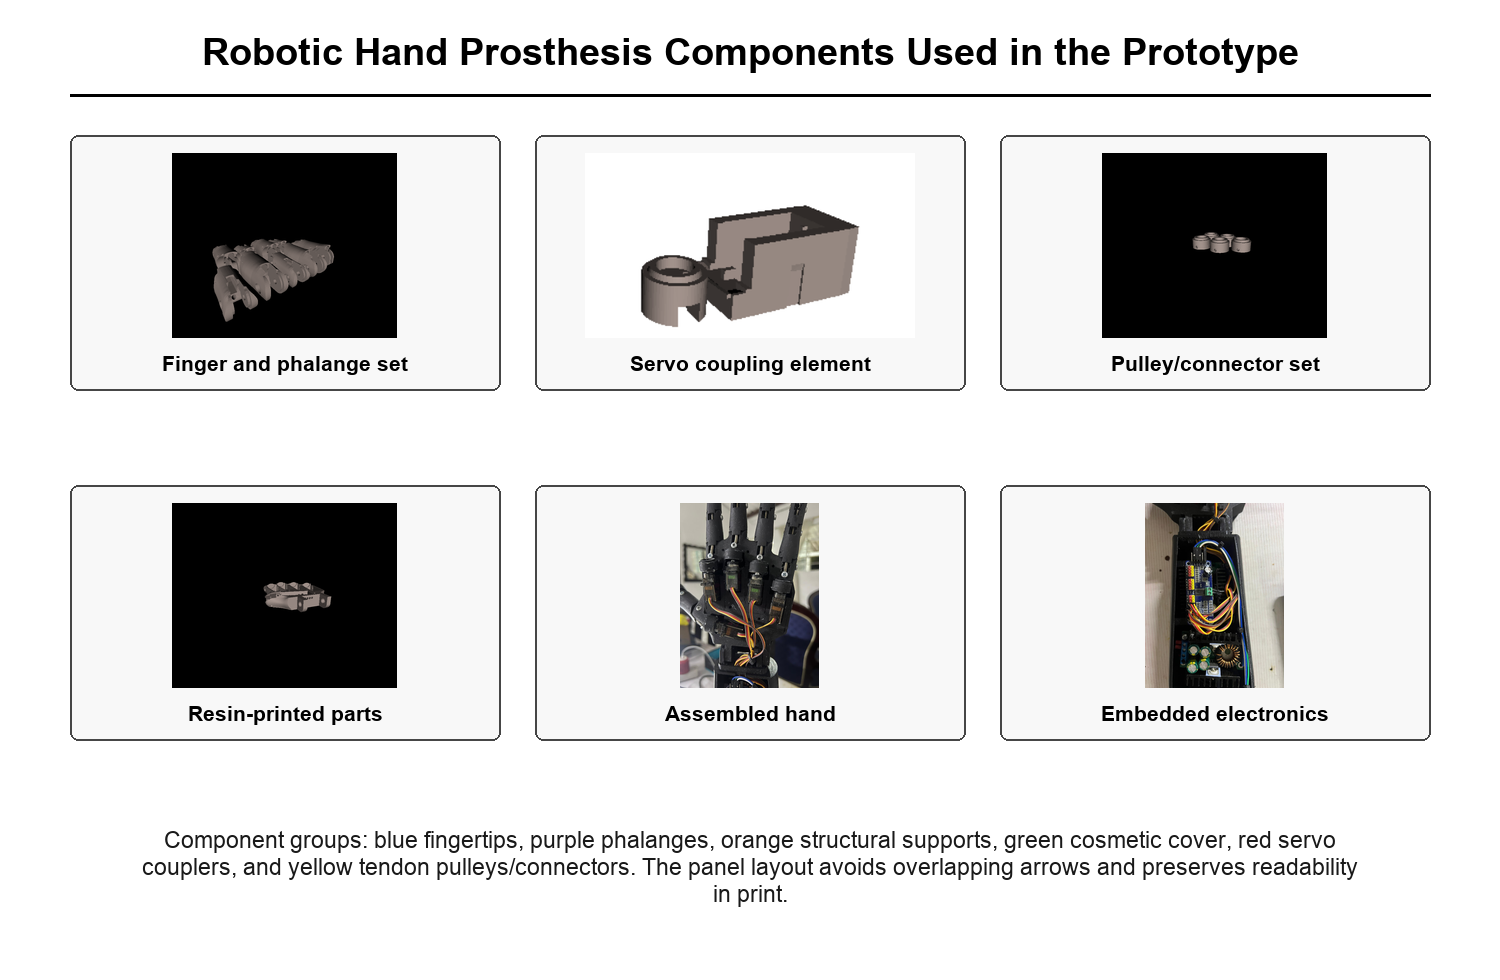
\includegraphics[width=0.82\linewidth]{fig03_prosthesis_components.png}
\caption{Main mechanical components of the robotic hand prosthesis, including finger segments, palm structure, tendon-transmission elements, servomotor supports and forearm housing.\label{fig:prosthesis-components}}
\end{figure}

Recognized classes were mapped to predefined finger-position vectors: rest, open hand, closed fist, pinch and object grasp.

To avoid abrupt movements, servo positions are updated progressively through incremental PWM interpolation. The power stage uses an 11.1 V, 2200 mAh LiPo battery and independent XL4016 DC--DC regulators to separate embedded control from servomotor supply, reducing voltage drops during coordinated activation.

\subsection{Evaluation Metrics}

Offline classification was evaluated using accuracy, precision, recall and F1-score. For class $m$, the metrics are defined as
\begin{equation}
    \label{eq:precision-recall}
    \mathrm{Precision}_m = \frac{TP_m}{TP_m+FP_m},
    \quad
    \mathrm{Recall}_m = \frac{TP_m}{TP_m+FN_m},
\end{equation}
\begin{equation}
    \label{eq:f1-accuracy}
    \mathrm{F1}_m =
    \frac{2\,\mathrm{Precision}_m\,\mathrm{Recall}_m}
    {\mathrm{Precision}_m+\mathrm{Recall}_m},
    \quad
    \mathrm{Accuracy} =
    \frac{\sum_m TP_m}{N_{\mathrm{test}}},
\end{equation}
where $TP_m$, $FP_m$ and $FN_m$ denote class-specific true positives, false positives and false negatives. Equations~\eqref{eq:precision-recall} and~\eqref{eq:f1-accuracy} define the supervised offline metrics, with macro averages weighted equally across classes.

To support analysis of class separability in the EMG feature space, the Fisher discriminant ratio can be computed from a feature representation $\boldsymbol{\phi}_{i}$ extracted from each window:
\begin{equation}
    \label{eq:fisher-ratio}
    J_{\mathrm{F}}
    =
    \frac{\operatorname{tr}(\mathbf{S}_{B})}
    {\operatorname{tr}(\mathbf{S}_{W})},
\end{equation}
where $\mathbf{S}_{B}$ and $\mathbf{S}_{W}$ are the between-class and within-class scatter matrices, respectively. These matrices are defined as
\begin{equation}
    \label{eq:scatter-matrices}
    \mathbf{S}_{B}
    =
    \sum_{m=1}^{M}
    N_m
    (\boldsymbol{\mu}_{m}-\boldsymbol{\mu})
    (\boldsymbol{\mu}_{m}-\boldsymbol{\mu})^{\top},
    \quad
    \mathbf{S}_{W}
    =
    \sum_{m=1}^{M}
    \sum_{\boldsymbol{\phi}_{i}\in m}
    (\boldsymbol{\phi}_{i}-\boldsymbol{\mu}_{m})
    (\boldsymbol{\phi}_{i}-\boldsymbol{\mu}_{m})^{\top}.
\end{equation}
A larger Equation~\eqref{eq:fisher-ratio}, computed from Equation~\eqref{eq:scatter-matrices}, indicates stronger separation between gesture classes relative to within-class variability, supporting future reproducibility analyses of whether high accuracy reflects separable EMG structure.

Embedded operation was evaluated using model confidence, instantaneous/smoothed prediction agreement and temporal stability. Let $\hat{y}_k$ be the instantaneous prediction and $\bar{y}_k$ the smoothed prediction. Agreement was computed as
\begin{equation}
    \label{eq:agreement}
    A =
    \frac{1}{K_{\mathrm{rt}}}
    \sum_{k=1}^{K_{\mathrm{rt}}}
    \mathbb{I}\left(\hat{y}_k=\bar{y}_k\right),
\end{equation}
where $K_{\mathrm{rt}}$ is the number of real-time predictions and $\mathbb{I}(\cdot)$ is the indicator function. Temporal stability was
\begin{equation}
    \label{eq:stability}
    S =
    \frac{1}{K_{\mathrm{rt}}-1}
    \sum_{k=2}^{K_{\mathrm{rt}}}
    \mathbb{I}\left(\bar{y}_k=\bar{y}_{k-1}\right).
\end{equation}
Because continuous ground truth was not recorded during embedded operation, Equations~\eqref{eq:confidence}, \eqref{eq:posterior-entropy}, \eqref{eq:agreement} and~\eqref{eq:stability} quantify implementation behavior rather than supervised online accuracy.

\section{Experimental Validation and Results}

\subsection{Offline Classification Performance}

The CNN--BiLSTM classifier was evaluated using an independent test set of 496 segmented windows not used during model fitting or hyperparameter selection. The model achieved a global accuracy of 0.9959 and macro-averaged precision, recall and F1-score values of 0.9958. Table~\ref{tab:classification} reports the per-class metrics.

\begin{table}[H]
\centering
\caption{Classification performance on the test set.\label{tab:classification}}
\begin{tabular}{lcccc}
\toprule
\textbf{Class} & \textbf{Precision} & \textbf{Recall} & \textbf{F1-score} & \textbf{Support} \\
\midrule
Object grasp & 1.0000 & 1.0000 & 1.0000 & 106 \\
Open hand & 0.9859 & 0.9859 & 0.9859 & 71 \\
Pinch & 0.9929 & 0.9929 & 0.9929 & 141 \\
Closed fist & 1.0000 & 1.0000 & 1.0000 & 71 \\
Rest & 1.0000 & 1.0000 & 1.0000 & 107 \\
\midrule
Global accuracy & -- & -- & 0.9960 & 496 \\
Macro average & 0.9958 & 0.9958 & 0.9958 & 496 \\
\bottomrule
\end{tabular}
\end{table}

Most errors were concentrated between open hand and pinch, a physiologically plausible confusion because both gestures can involve overlapping forearm extensor/flexor activation. The error pattern therefore suggests localized ambiguity between biomechanically similar classes rather than global model instability.

\subsection{Training Dynamics and Generalization Behavior}

The training curves in Figure~\ref{fig:training-dynamics} showed rapid early improvement, stabilization near maximum accuracy and convergence without substantial train-validation divergence. This supports stable optimization under the selected preprocessing, class weighting and label-smoothing strategy. Because data came from one participant under controlled posture and electrode placement, the result supports intra-subject feasibility rather than population-level generalization.

\begin{figure}[H]
\centering
\begin{minipage}{0.49\linewidth}
\centering
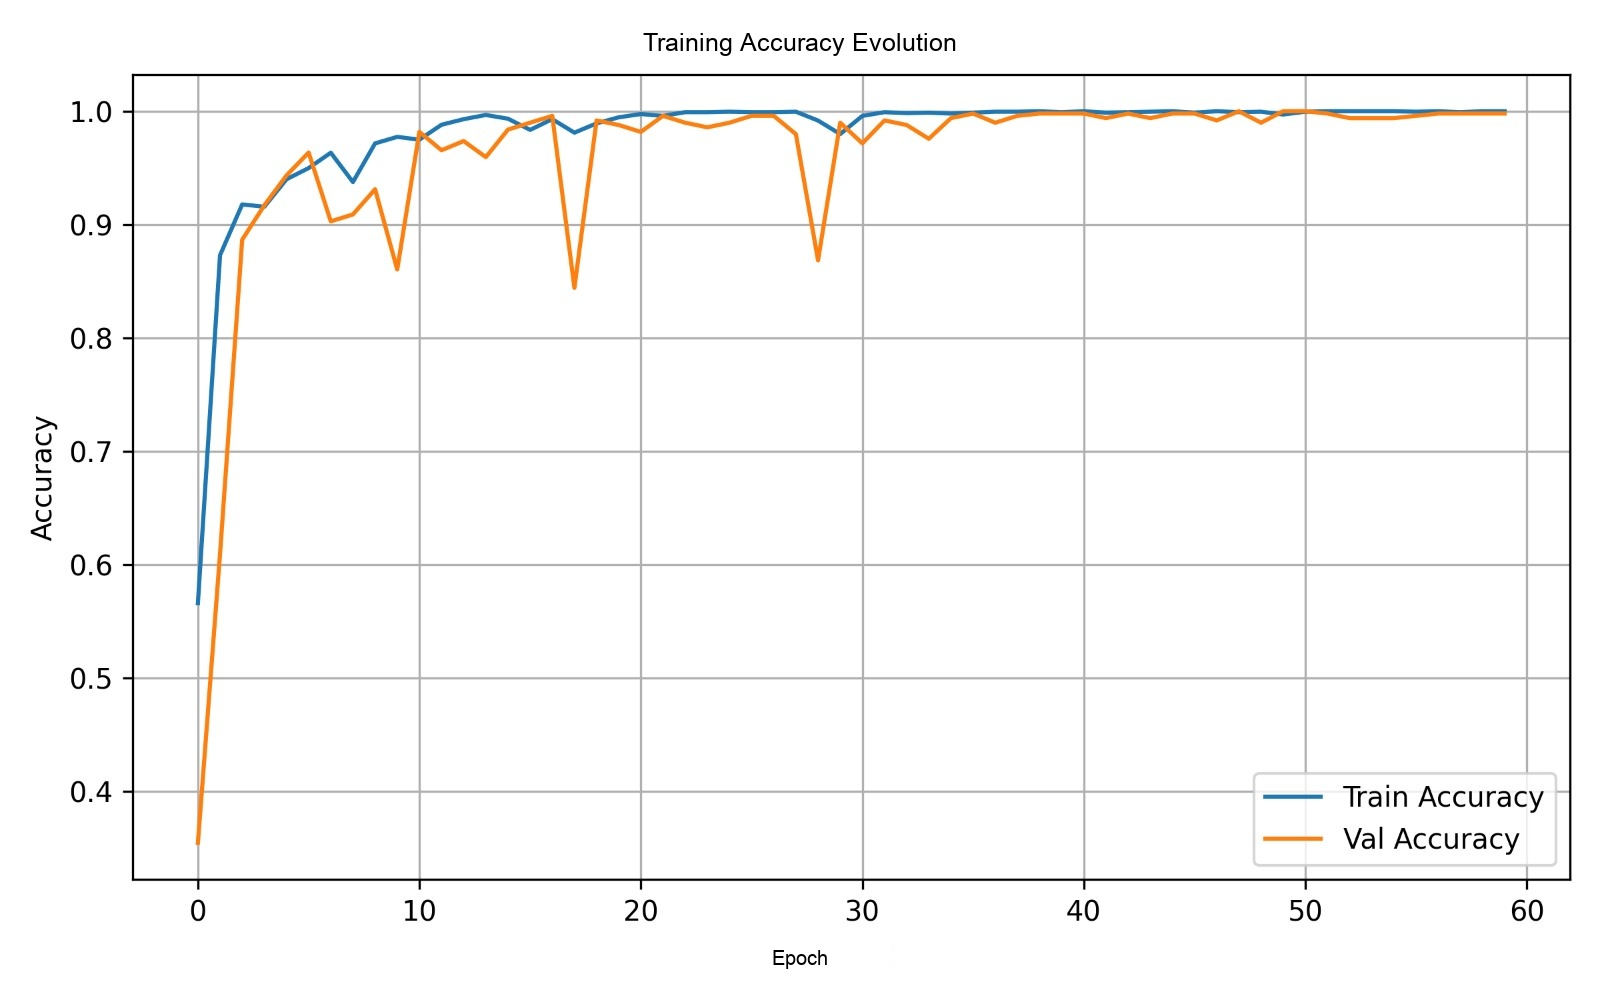
\includegraphics[width=\linewidth]{fig05_training_accuracy.jpeg}
\end{minipage}
\hfill
\begin{minipage}{0.49\linewidth}
\centering
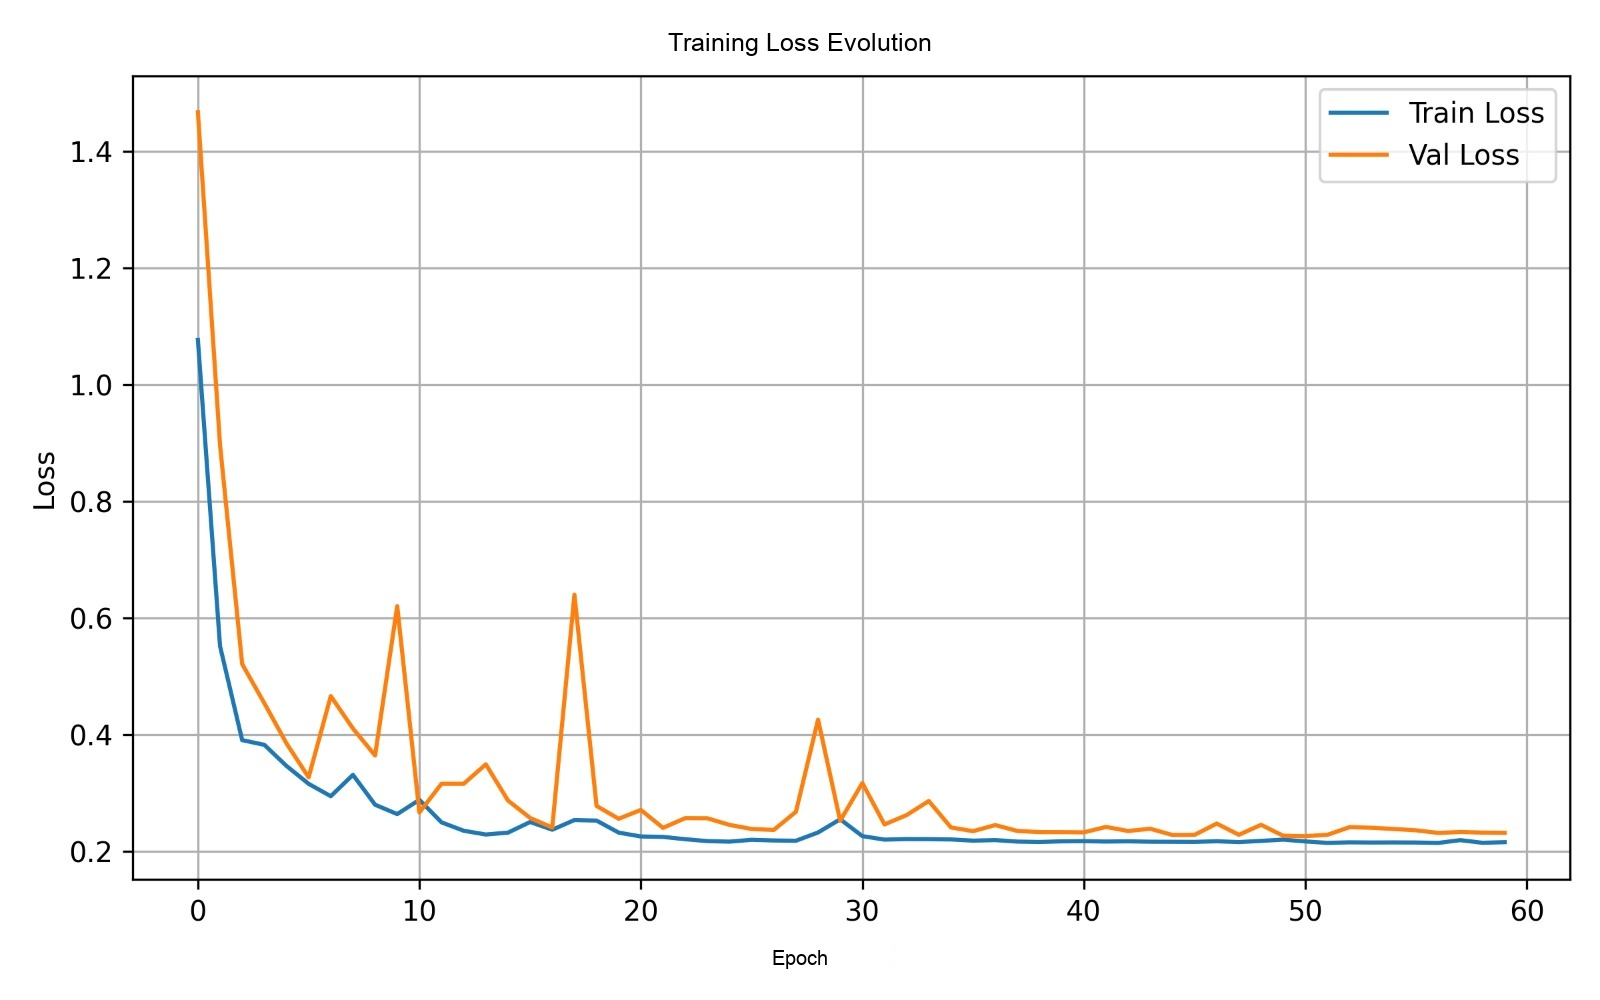
\includegraphics[width=\linewidth]{fig06_training_loss.jpeg}
\end{minipage}
\caption{Training dynamics of the CNN--BiLSTM model: accuracy and loss curves over 60 epochs show rapid convergence and stable validation behavior under the selected preprocessing and training strategy.\label{fig:training-dynamics}}
\end{figure}

\subsection{Real-Time Embedded Operation}

The embedded system was evaluated during continuous operation on the Raspberry Pi. A total of 199 predictions were registered over 44.5 s. Table~\ref{tab:realtime} summarizes the real-time indicators.

\begin{table}[H]
\centering
\caption{Real-time inference indicators recorded during embedded operation.\label{tab:realtime}}
\begin{tabular}{lc}
\toprule
\textbf{Indicator} & \textbf{Value} \\
\midrule
Registered predictions & 199 \\
Test duration & 44.5 s \\
Mean confidence & 0.9015 \\
Median confidence & 0.9589 \\
Minimum confidence & 0.3957 \\
Maximum confidence & 0.9770 \\
Instantaneous/smoothed prediction agreement & 85.9\% \\
Class transitions & 22 \\
Transition rate & 11.1\% \\
\bottomrule
\end{tabular}
\end{table}

The high median confidence indicates strong certainty for most windows, while lower-confidence intervals are consistent with gesture transitions or inconsistent contractions. The 85.9\% instantaneous/smoothed agreement and 11.1\% transition rate support temporal smoothing as an embedded-stabilization mechanism. Because synchronized real-time labels were unavailable, these are operability metrics rather than supervised online accuracy.

\subsection{Functional Prosthesis Validation}

Functional validation integrated the trained model, PWM stage and robotic hand. Under controlled execution of the five gestures, the system translated stabilized predictions into the expected postures: neutral, open hand, closed fist, pinch and object grasp. Quantitative indicators are summarized in Table~\ref{tab:functional}.

\begin{table}[H]
\centering
\caption{Functional validation metrics from continuous real-time prediction analysis.\label{tab:functional}}
\begin{tabularx}{\textwidth}{llX}
\toprule
\textbf{Metric} & \textbf{Value} & \textbf{Description} \\
\midrule
Total predictions & 199 & Number of real-time instances analyzed \\
Temporal stability & 88.9\% & Consecutive predictions that remained consistent \\
Transitions between classes & 11.1\% & Changes between consecutive predictions \\
Window size & 0.75 s & Duration of the analysis window \\
Update step & 0.1 s & Real-time prediction update interval \\
\bottomrule
\end{tabularx}
\end{table}

The system operated without observed interruptions in acquisition, inference or actuation. Perceived latency was suitable for real-time interaction, and progressive PWM interpolation avoided abrupt movements. Figure~\ref{fig:functional-validation} shows the integrated functional operation.

\begin{figure}[H]
\centering
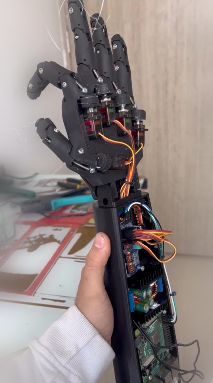
\includegraphics[width=0.42\linewidth]{fig07_functional_validation.png}
\caption{Functional validation of the complete system during gesture-driven prosthetic operation, showing the integrated interaction between EMG acquisition, embedded inference and robotic-hand actuation.\label{fig:functional-validation}}
\end{figure}

Table~\ref{tab:validation_scope} summarizes the validation scope relative to the controls that remain necessary before translational claims. This distinction is included to separate demonstrated evidence from future generalization tests.

\begin{table}[H]
\centering
\caption{Validation scope of the present study and controls required for broader generalization.\label{tab:validation_scope}}
\begin{tabularx}{\textwidth}{lXX}
\toprule
\textbf{Validation axis} & \textbf{Implemented in this study} & \textbf{Required next control} \\
\midrule
Offline classifier & Independent intra-subject test windows; accuracy, precision, recall and F1-score & Cross-session and cross-user testing \\
Embedded inference & TensorFlow Lite operation on Raspberry Pi; confidence, agreement and stability & Latency distribution and synchronized online labels \\
Decision stabilization & Majority-vote smoothing and progressive PWM interpolation & Comparison against no-smoothing and alternative smoothing rules \\
Functional actuation & Five gesture-to-posture mappings on the robotic hand & Standardized task success, grasp force and finger kinematics \\
\bottomrule
\end{tabularx}
\end{table}

\section{Discussion}

The main finding is that a low-cost embedded platform can execute the complete myoelectric-control chain: acquisition, causal filtering, deep-learning inference, temporal decision stabilization and physical prosthetic actuation. The 99.6\% offline accuracy is consistent with recent sEMG deep-learning studies \cite{Nahid2020Myo,Chung2019Myo,Celik2026,Tsinganos2018,Shanmuganathan2023}, but the contribution is the integration of a mathematically defined classifier into an edge-deployed assistive-technology pipeline evaluated with both classification and embedded-operation indicators.

The CNN--BiLSTM architecture matches the signal structure: convolutions capture local activation motifs, the envelope branch contributes contraction-intensity information, and the BiLSTM models within-window temporal dependencies before the softmax decision. Temporal smoothing is also control-relevant: without it, isolated misclassifications can produce unwanted finger motion. The majority-vote strategy reduced short-term fluctuations while preserving a 0.1 s update step, and PWM interpolation improved mechanical smoothness by avoiding instantaneous servo jumps.

The prototype addresses accessibility by combining a low-cost sEMG armband, Raspberry Pi processing, TensorFlow Lite inference, MG90S servomotors, 3D-printed structures and open-source mechanical design. Nevertheless, the evidence remains controlled and intra-subject. Data were acquired from one participant; sEMG varies with anatomy, electrode displacement, fatigue, sweating, skin impedance and donning conditions. Real-time evaluation used confidence, agreement and stability because synchronized online labels were not recorded, and functional validation did not quantify grasp force, finger kinematics or standardized task success.

Future work should collect multi-participant and amputee-user data across sessions, compare compact architectures and quantized models, synchronize online labels, measure latency distributions and incorporate force or position feedback for adaptive grasp control. These steps are required before clinical or daily-use claims can be made.

\section{Conclusions}

This study presented a formalized embedded deep-learning pipeline for real-time control of a robotic hand prosthesis using eight-channel sEMG. The system integrates Myo Armband acquisition, causal filtering, sliding-window segmentation, z-score normalization, CNN--BiLSTM classification, TensorFlow Lite inference, majority-vote stabilization and PWM actuation. The model reached 99.6\% test accuracy and 99.58\% macro F1-score, while embedded validation showed stable continuous operation and coherent gesture-to-motion mapping. The findings support accessible edge-AI architectures for myoelectric assistive technologies, but the work should be interpreted as a controlled intra-subject proof-of-concept pending multi-user, amputee-user, cross-session and biomechanical validation.

\section*{Patents}

No patents resulting from this work are reported in this manuscript draft.

\supplementary{The following supporting materials should be submitted with the article to maximize reproducibility: acquisition script, preprocessing configuration, channel-wise normalization constants, class-index mapping, trained TensorFlow Lite model, embedded-inference pseudocode, PWM gesture map, model-training logs and CAD/prototype assembly files.}

\authorcontributions{Conceptualization, R.Y.A.S., Y.C.B.A., J.J.L.M., C.H.V.N. and C.J.G.L.; methodology, R.Y.A.S., Y.C.B.A. and J.J.L.M.; software, R.Y.A.S., Y.C.B.A. and J.J.L.M.; validation, R.Y.A.S., Y.C.B.A. and J.J.L.M.; formal analysis, R.Y.A.S., Y.C.B.A., J.J.L.M. and C.H.V.N.; investigation, R.Y.A.S., Y.C.B.A. and J.J.L.M.; resources, C.H.V.N. and C.J.G.L.; data curation, R.Y.A.S., Y.C.B.A. and J.J.L.M.; writing--original draft preparation, R.Y.A.S., Y.C.B.A. and J.J.L.M.; writing--review and editing, C.H.V.N. and C.J.G.L.; visualization, R.Y.A.S., Y.C.B.A. and J.J.L.M.; supervision, C.H.V.N. and C.J.G.L.; project administration, C.H.V.N. All authors have read and agreed to the published version of the manuscript.}

\conflictsofinterest{The authors declare no conflict of interest.}

\section*{Nomenclature}

\begin{tabularx}{0.94\linewidth}{lX}
\toprule
\textbf{Symbol or acronym} & \textbf{Meaning} \\
\midrule
sEMG & Surface electromyography \\
CNN & Convolutional neural network \\
BiLSTM & Bidirectional long short-term memory network \\
PWM & Pulse-width modulation \\
$C$ & Number of EMG channels \\
$W$ & Window length in samples \\
$H$ & Sliding-window hop size \\
$K$ & Number of predictions used for temporal stabilization \\
$\mathbf{x}[n]$ & Multichannel EMG sample at index $n$ \\
$\mathbf{X}_k$ & Segmented EMG window \\
$\mathbf{p}_k$ & Posterior class-probability vector \\
$\hat{y}_k$ & Instantaneous predicted gesture class \\
$\bar{y}_k$ & Temporally stabilized gesture class \\
$\mathbf{q}^{\star}_k$ & Desired prosthetic finger-position vector \\
$u_{i,k}$ & PWM command for servo $i$ \\
$T_{\mathrm{total}}$ & End-to-end response time \\
\bottomrule
\end{tabularx}

\reftitle{References}


\begin{thebibliography}{999}

\bibitem{Dunai2025Tech}
Dunai, L.; Segui Verdu, I.; Turcanu, D. Prosthetic hand based on human hand anatomy controlled by surface electromyography and artificial neural networks. \textit{Technologies} \textbf{2025}, \textit{13}, 21. \url{https://doi.org/10.3390/technologies13010021}.

\bibitem{Covaciu2025Tech}
Covaciu, F.; Gherman, B.; Vaida, C. A combined mirror--EMG robot-assisted therapy system for lower limb rehabilitation. \textit{Technologies} \textbf{2025}, \textit{13}, 227. \url{https://doi.org/10.3390/technologies13060227}.

\bibitem{Lotfi2018Tech}
Lotfi, A.; Langensiepen, C.; Yahaya, S.W. Socially assistive robotics: Robot exercise trainer for older adults. \textit{Technologies} \textbf{2018}, \textit{6}, 32. \url{https://doi.org/10.3390/technologies6010032}.

\bibitem{Stasolla2023Tech}
Stasolla, F.; Lopez, A.; Akbar, K. Matching assistive technology, telerehabilitation, and virtual reality to promote cognitive rehabilitation. \textit{Technologies} \textbf{2023}, \textit{11}, 43. \url{https://doi.org/10.3390/technologies11020043}.

\bibitem{Bush2024Tech}
Bush, J.; Benham, S.; Kaniamattam, M. Development and evaluation of an mHealth app that promotes access to 3D printable assistive devices. \textit{Technologies} \textbf{2024}, \textit{12}, 114. \url{https://doi.org/10.3390/technologies12070114}.

\bibitem{Giansanti2025Tech}
Giansanti, D. Empowering independence: The role of assistive technologies in enhancing quality of life. \textit{Technologies} \textbf{2025}, \textit{13}, 408. \url{https://doi.org/10.3390/technologies13090408}.

\bibitem{Manakitsa2024Tech}
Manakitsa, N.; Maraslidis, G.S.; Moysis, L. A review of machine learning and deep learning for object detection, semantic segmentation, and human action recognition. \textit{Technologies} \textbf{2024}, \textit{12}, 15. \url{https://doi.org/10.3390/technologies12020015}.

\bibitem{Percuku2025Tech}
Percuku, A.; Minkovska, D.; Hinov, N. Enhancing electricity load forecasting with machine learning and deep learning. \textit{Technologies} \textbf{2025}, \textit{13}, 59. \url{https://doi.org/10.3390/technologies13020059}.

\bibitem{Jalloul2025Tech}
Jalloul, R.; Krishnappa, C.H.; Agughasi, V.I. Enhancing early breast cancer detection with infrared thermography: A comparative evaluation of deep learning approaches. \textit{Technologies} \textbf{2025}, \textit{13}, 7. \url{https://doi.org/10.3390/technologies13010007}.

\bibitem{Kouretas2020Tech}
Kouretas, I.; Paliouras, V. Hardware implementation of a softmax-like function for deep learning. \textit{Technologies} \textbf{2020}, \textit{8}, 46. \url{https://doi.org/10.3390/technologies8030046}.

\bibitem{Kraft2020Tech}
Kraft, D.; Srinivasan, K.; Bieber, G. Deep learning based fall detection algorithms for embedded systems, smartwatches, and IoT devices using accelerometers. \textit{Technologies} \textbf{2020}, \textit{8}, 72. \url{https://doi.org/10.3390/technologies8040072}.

\bibitem{Sanida2022Tech}
Sanida, T.; Sideris, A.; Tsiktsiris, D. Lightweight neural network for COVID-19 detection from chest X-ray images implemented on an embedded system. \textit{Technologies} \textbf{2022}, \textit{10}, 37. \url{https://doi.org/10.3390/technologies10020037}.

\bibitem{Farina2014}
Farina, D.; Jiang, N.; Rehbaum, H.; Holobar, A.; Graimann, B.; Dietl, H.; Aszmann, O. The extraction of neural information from the surface EMG for the control of upper-limb prostheses: Emerging avenues and challenges. \textit{IEEE Trans. Neural Syst. Rehabil. Eng.} \textbf{2014}, \textit{22}, 797--809. \url{https://doi.org/10.1109/TNSRE.2014.2305111}.

\bibitem{Englehart2003}
Englehart, K.; Hudgins, B. A robust, real-time control scheme for multifunction myoelectric control. \textit{IEEE Trans. Biomed. Eng.} \textbf{2003}, \textit{50}, 848--854. \url{https://doi.org/10.1109/TBME.2003.813539}.

\bibitem{Hudgins1993}
Hudgins, B.; Parker, P.; Scott, R.N. A new strategy for multifunction myoelectric control. \textit{IEEE Trans. Biomed. Eng.} \textbf{1993}, \textit{40}, 82--94. \url{https://doi.org/10.1109/10.204774}.

\bibitem{Ha2011}
Ha, K.H.; Varol, H.A.; Goldfarb, M. Volitional control of a prosthetic knee using surface electromyography. \textit{IEEE Trans. Biomed. Eng.} \textbf{2011}, \textit{58}, 144--151. \url{https://doi.org/10.1109/TBME.2010.2070840}.

\bibitem{Kuiken2009}
Kuiken, T.A.; Li, G.; Lock, B.A.; Lipschutz, R.D.; Miller, L.A.; Stubblefield, K.A.; Englehart, K.B. Targeted muscle reinnervation for real-time myoelectric control of multifunction artificial arms. \textit{JAMA} \textbf{2009}, \textit{301}, 619--628. \url{https://doi.org/10.1001/jama.2009.116}.

\bibitem{Cipriani2011}
Cipriani, C.; Antfolk, C.; Controzzi, M.; Lundborg, G.; Rosen, B.; Carrozza, M.C.; Sebelius, F. Online myoelectric control of a dexterous hand prosthesis by transradial amputees. \textit{IEEE Trans. Neural Syst. Rehabil. Eng.} \textbf{2011}, \textit{19}, 260--270. \url{https://doi.org/10.1109/TNSRE.2011.2108667}.

\bibitem{Oskoei2007}
Oskoei, M.A.; Hu, H. Myoelectric control systems--A survey. \textit{Biomed. Signal Process. Control} \textbf{2007}, \textit{2}, 275--294. \url{https://doi.org/10.1016/j.bspc.2007.07.009}.

\bibitem{Scheme2011}
Scheme, E.; Englehart, K. Electromyogram pattern recognition for control of powered upper-limb prostheses: State of the art and challenges for clinical use. \textit{J. Rehabil. Res. Dev.} \textbf{2011}, \textit{48}, 643--660. \url{https://doi.org/10.1682/JRRD.2010.09.0177}.

\bibitem{Chowdhury2013}
Chowdhury, R.H.; Reaz, M.B.I.; Ali, M.A.B.M.; Bakar, A.A.A.; Chellappan, K.; Chang, T.G. Surface electromyography signal processing and classification techniques. \textit{Sensors} \textbf{2013}, \textit{13}, 12431--12466. \url{https://doi.org/10.3390/s130912431}.

\bibitem{Phinyomark2012}
Phinyomark, A.; Phukpattaranont, P.; Limsakul, C. Feature reduction and selection for EMG signal classification. \textit{Expert Syst. Appl.} \textbf{2012}, \textit{39}, 7420--7431. \url{https://doi.org/10.1016/j.eswa.2012.01.102}.

\bibitem{Merletti1997}
Merletti, R.; Lo Conte, L. Surface EMG signal processing during isometric contractions. \textit{J. Electromyogr. Kinesiol.} \textbf{1997}, \textit{7}, 241--250. \url{https://doi.org/10.1016/S1050-6411(97)00010-2}.

\bibitem{Atzori2014SciData}
Atzori, M.; Gijsberts, A.; Castellini, C.; Caputo, B.; Hager, A.G.M.; Elsig, S.; Giatsidis, G.; Bassetto, F.; Muller, H. Electromyography data for non-invasive naturally-controlled robotic hand prostheses. \textit{Sci. Data} \textbf{2014}, \textit{1}, 140053. \url{https://doi.org/10.1038/sdata.2014.53}.

\bibitem{NinaPro2015}
Atzori, M.; Gijsberts, A.; Heynen, S.; Hager, A.G.M.; Deriaz, O.; Van Der Smagt, P.; Castellini, C.; Caputo, B.; Muller, H. The Ninapro database: A resource for sEMG naturally controlled robotic hand prosthetics. In \textit{Proceedings of the 37th Annual International Conference of the IEEE Engineering in Medicine and Biology Society}; Milan, Italy, 2015; pp. 7151--7154. \url{https://doi.org/10.1109/EMBC.2015.7320041}.

\bibitem{Muceli2013}
Muceli, S. \textit{Multi-Channel Surface Electromyography for Simultaneous and Proportional Control of Prostheses}; River Publishers: Aalborg, Denmark, 2013. \url{https://doi.org/10.13052/rp-9788793102361}.

\bibitem{Prakash2021}
Prakash, A.; Sharma, S. Single-channel surface electromyography (sEMG) based control of a multi-functional prosthetic hand. \textit{Instrum. Sci. Technol.} \textbf{2021}, \textit{49}, 1--18. \url{https://doi.org/10.1080/10739149.2021.1880933}.

\bibitem{He2017Myo}
He, J.; Yang, X.; Wang, X. Hand gesture recognition using MYO armband. In \textit{Proceedings of the 2017 Chinese Automation Congress}; Jinan, China, 2017; pp. 4850--4855. \url{https://doi.org/10.1109/CAC.2017.8243637}.

\bibitem{Kaya2018Myo}
Kaya, O.; Kumbasar, T. Hand gesture recognition systems with the wearable Myo Armband. In \textit{Proceedings of the 2018 6th International Conference on Control Engineering and Information Technology}; Istanbul, Turkey, 2018. \url{https://doi.org/10.1109/CEIT.2018.8751927}.

\bibitem{Sathiyanarayanan2016Myo}
Sathiyanarayanan, M.; Rajan, S. MYO Armband for physiotherapy healthcare: A case study using gesture recognition application. In \textit{Proceedings of the 2016 8th International Conference on Communication Systems and Networks}; Bangalore, India, 2016. \url{https://doi.org/10.1109/COMSNETS.2016.7439933}.

\bibitem{Boyali2015Myo}
Boyali, A.; Hashimoto, N.; Matsumoto, O. Hand posture and gesture recognition using MYO armband and spectral collaborative representation based classification. In \textit{Proceedings of the 2015 IEEE 4th Global Conference on Consumer Electronics}; Osaka, Japan, 2015. \url{https://doi.org/10.1109/GCCE.2015.7398619}.

\bibitem{Benalcazar2017Myo}
Benalcazar, M.E.; Jaramillo, A.G.; Zea, J.A.; Paez, A.; Andaluz, V.H. Hand gesture recognition using machine learning and the Myo armband. In \textit{Proceedings of the 25th European Signal Processing Conference}; Kos, Greece, 2017. \url{https://doi.org/10.23919/EUSIPCO.2017.8081366}.

\bibitem{Chung2019Myo}
Chung, E.A.; Benalcazar, M.E. Real-time hand gesture recognition model using deep learning techniques and EMG signals. In \textit{Proceedings of the 27th European Signal Processing Conference}; A Coruna, Spain, 2019. \url{https://doi.org/10.23919/EUSIPCO.2019.8903136}.

\bibitem{Nahid2020Myo}
Nahid, A.A.; Rahman, M.M.; Ahad, M.A.R. Deep learning based surface EMG hand gesture classification for low-cost myoelectric prosthetic control. In \textit{Proceedings of the Joint 9th International Conference on Informatics, Electronics and Vision and 4th International Conference on Imaging, Vision and Pattern Recognition}; Kitakyushu, Japan, 2020. \url{https://doi.org/10.1109/ICIEVicIVPR48672.2020.9306613}.

\bibitem{LeCun2015}
LeCun, Y.; Bengio, Y.; Hinton, G. Deep learning. \textit{Nature} \textbf{2015}, \textit{521}, 436--444. \url{https://doi.org/10.1038/nature14539}.

\bibitem{Hochreiter1997}
Hochreiter, S.; Schmidhuber, J. Long short-term memory. \textit{Neural Comput.} \textbf{1997}, \textit{9}, 1735--1780. \url{https://doi.org/10.1162/neco.1997.9.8.1735}.

\bibitem{Tsinganos2018}
Tsinganos, P.; Cornelis, B.; Cornelis, J.; Jansen, B.; Skodras, A. Deep learning in EMG-based gesture recognition. In \textit{Proceedings of the 5th International Conference on Physiological Computing Systems}; Seville, Spain, 2018; pp. 107--114. \url{https://doi.org/10.5220/0006960201070114}.

\bibitem{Celik2026}
Celik, Y.; Can, O. Surface EMG-based hand gesture recognition using a hybrid multistream deep learning architecture. \textit{Sensors} \textbf{2026}, \textit{26}, 2281. \url{https://doi.org/10.3390/s26072281}.

\bibitem{Shanmuganathan2023}
Shanmuganathan, V.; Barbosa, P.C.; da Cunha Neto, J.S.; Zhang, L.; de Albuquerque, V.H.C.; Pasupathi, S. Development of intelligent and integrated technology for pattern recognition in EMG signals for robotic prosthesis command. \textit{Expert Syst.} \textbf{2023}, \textit{40}, e13109. \url{https://doi.org/10.1111/exsy.13109}.

\bibitem{Zaman2020TFLite}
Zaman, N. \textit{TensorFlow Lite for Mobile Development}; Apress: Berkeley, CA, USA, 2020. \url{https://doi.org/10.1007/978-1-4842-6666-3}.

\end{thebibliography}

\end{document}
